We instantiated the above described algorithm in the context of logic grid puzzles. 
In that setting there are basically three types of constraints in $\allconstraints$: transitivity constraints, bijectivity constraints and clues, where the first two follow the same structure in every puzzle and the clues are obtained in a mostly automatic way (see Section \ref{sec:holistic}). 
Before defining a cost-function, and the estimation for $g$ used in our implementation, we provide some observation that drove our design decision. 

\textbf{Observation 1: propagations from a single implicit constraint are very easy to understand} Contrary to the clues, the implicit constraints (transitivity/bijectivity) are very limited in form and propagations over them follow well-specified patterns. 
For instance in the case of bijectivity, a typical pattern that occurs is that when $X-1$ out of $X$ possible values for a given function have been derived not to be possible, it is propagated that the last value should be true; this is visualized for instance in Figure \ref{fig:zebrascreen}. 
Hence, in our implementation, we ensure that they are always performed first. Stated differently, $g$ and $f$ are designed in such a way that $g(S_1)\geq f(I,S_2)$ whenever $S_2$ consists of only one implicit constraint and $S_1$ does not. 

\textbf{Observation 2: clues propagate rarely by themselves}
We observed that the automatically obtained logic representation of clues usually has quite weak (unit) propagation strength in isolation. 
This is not a property of the clues, but rather of the final obtained translation. As an example, consider the following sentence: 
``The person who ordered capellini is either Damon or Claudia''. From this, a human reasoner might conclude that Angie did not order capellini. 
However, the obtained logical representation is 
\[\exists p: ordered(p,capellini)\land (p = Damon\lor p = Claudia).\]
This logic sentence only entails that Angie did not order capellini \emph{in conjunction with the bijectivity constraint on $ordered$}.
In the natural language sentence, this bijectivity is implicit by the use of \textbf{the} person which entails that there is only a single person ordering capellini. 

We observed that there is rarely any propagation from sole clues, and that only few implicit constraints are active together with a clue at any time. Hence, when pairing clues to other constraints we always pair it with the set of all implicit (bijectivity, transitivity) constraints.

\textbf{Observation 3: clues are typically used independently from other clues} 
A final observation is that in all the puzzles we encountered, human reasoners never needed to combine two clues in order to derive new information and that when such propagations are possible, they are quite hard to explain, and can be split up into derivations containing only single clues.
The latter is of course not guaranteed, since one can artificially devise disjunctive clues that do not allow propagation by themselves. 
Our algorithms are built to handle this case as well, but it turned out to be not necessary in practice. 

With these three observations in mind, we devised $f$ and $g$ as follows (where $nc(C)$ denotes the number of clues in $C$): \label{sec:cost}
\begin{align*}&f(I,C) = basecost(C) + |I| + |C|\\
&g(C) = basecost(C) = \left\{\begin{array}{ll}
                               0 & \text{if $|C|=1$ and $nc(C) = 0$}\\
                               20 & \text{if $|C|>1$ and $nc(C)=0$}\\
                               20\cdot nc(C) & \text{otherwise}
                              \end{array}\right.
                              \end{align*}
                              
The number $20$ is taken here to be larger than any reasonable explanation size. 
The effect of this,  is that we can generate our subsets $S$ in Line \ref{alg:min:for}
 of Algorithm \ref{alg:minexpl} in the following order:
\begin{compactitem}
 \item First all $S$ containing exactly one implicit constraint.
 \item Next, all $S$ containing exactly all implicit constraints and (optionally) exactly one clue.
 \item Finally, all clue pairs, triples etc. though in practice this is never reached.
\end{compactitem}
Summarized, our instantiation for logic grid puzzles differs from the generic methods developed in the previous section in that it uses a domain-specific optimization function $f$ and does not considering all $S$ in Line \ref{alg:min:for}, but only promising candidates based on our observations.

\begin{figure}[ht]
\centering
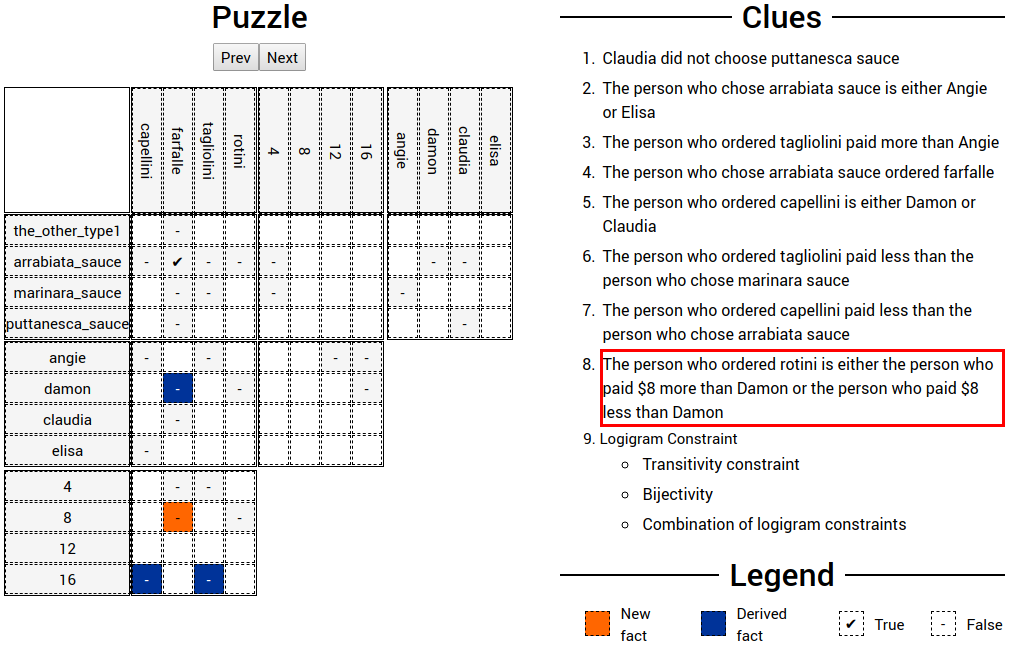
\includegraphics[width=\linewidth]{figures/zebra_screen_2}
\caption{Demonstration of hard explanation.}
\label{fig:screen2}
\end{figure}

For the complete non-redundant explanation sequence our tool produces on the running example using these scoring functions, we refer to \url{http://bartbog.github.io/zebra/pasta}. An example of the hardest derivation we encountered (with cost 28) is depicted in Figure \ref{fig:screen2}. It uses several bijectivity constraints for uniqueness of persons, but also for reasoning on the relation between costs and types of pasta, in combination with a clue and three assumptions.
Intuitively, the reasoning happening here can be explained as follows: if \textit{farfalle} were to cost \$8, then due to the assumptions and bijectivity \textit{rotini} would cost 16. However, since Damon did not take \textit{farfelle} (which we assumed costs \$8), this is in contradiction with the highlighted clue. Hence \textit{farfalle} does not cost \$8. 



\todo{add some observations for future work:
\begin{itemize}
 \item Nested explanation sometimes produces unused things. (max aggregates + greedy)
 \item Sometimes a nested explanation seems to difficult: could be made easier by using **more** clues, actually thus making the upper step harder. This suggests there might be a new way to define cost based on nested expl. 
\end{itemize}
}
